\section{Efficiency Analysis}

Given that this is a parallel algorithm, we would be remiss if we didn't study
it's efficiency. The classical method is an analysis via Amadahl's law, which
states that:
\[
  S_{{\rm latency}}(s) = \frac{1}{(1-p) + \frac{p}{s}}
\]
where $S_{{\rm latency}}$ is the theoretical speedup in execution of the whole
task, $s$ is the speedup of the portion benefiting from parallel processing, and
$p$ is the proportion of execution now being parallelized. Supposing we're
working on \hogwild\ with replacement, then the entire computation (minius I/O)
is parallelized, so $p = 1$. Furthermore, since the parallel region is just one
embarassingly parallel (after justification) loop, $s = P$, where $P$ is the
number of processors. Thus, Amadahl's law turns out to be pretty trivial in the
case of asynchronous stochastic methods, in that $S_{{\rm latency}}(s) = s = P$.

However, in practice this is most-definitely not observed, not in my tests, and
neither in the original paper \cite{2011NRRW}. See Figure \ref{fig:scaling} for
my scaling results.
\begin{figure}[!htb]
  \centering
  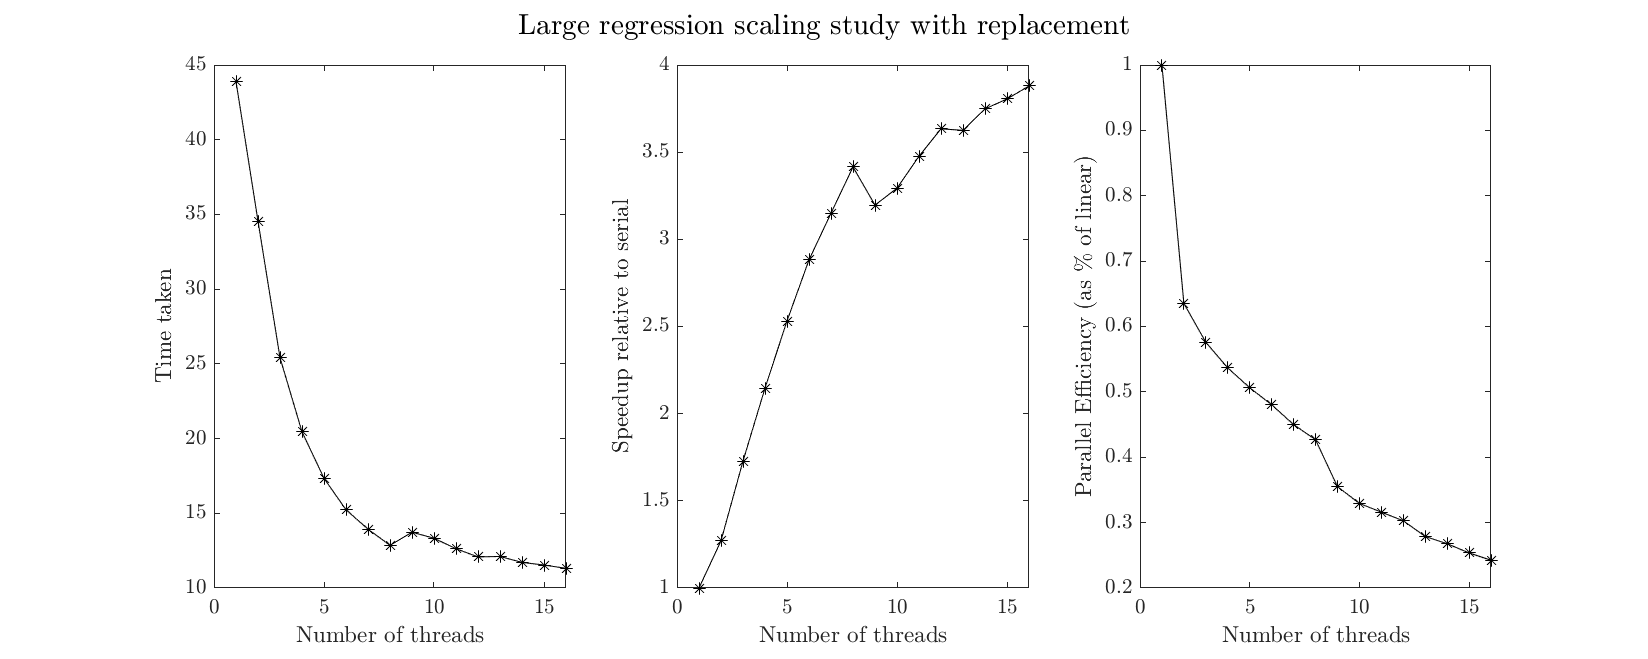
\includegraphics[width=1\textwidth]{./resources/replacement}
  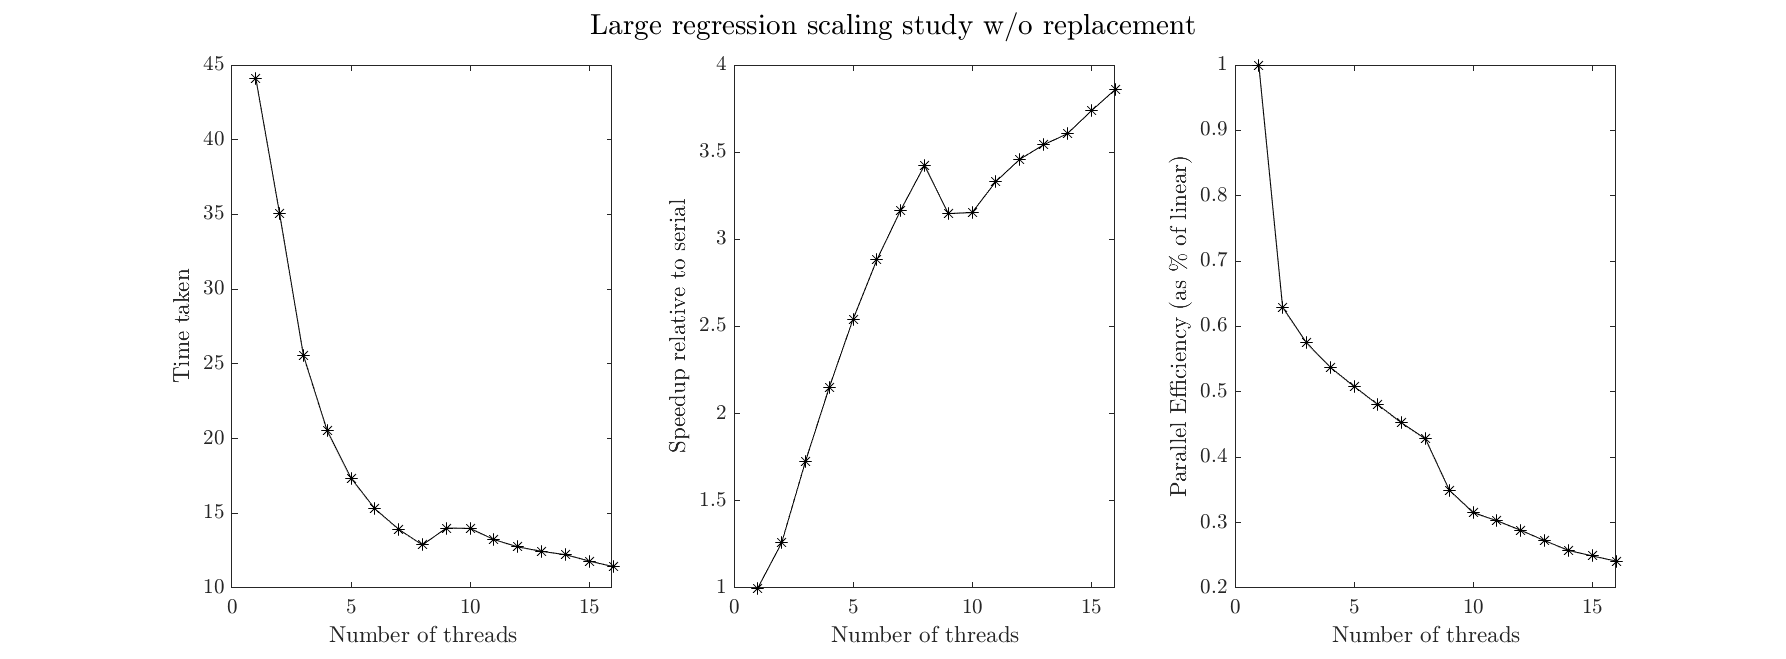
\includegraphics[width=1\textwidth]{./resources/noreplacement}
  \caption{
  } \label{fig:scaling}
\end{figure}
Specifically for my tests, it's not too hard to tell what's breaking the
performance. Simply put, we're being cruel to the cache. Both of these scaling
studies were computing over pretty large matrices, $A \in \mathbb{R}^{400^2
\times 400}$, which in just information is 0.5GB large. Furthermore, the column
of $400^2$ doubles, for my processor the Ryzen 3700X, doesn't even have a tenth
of it fit into L1 Cache. Thus for computing the gradient terms, which have
a $A_{i*}^T \cdot A_{i*}$ term inside of them, even if we explicity avoid
computing the full matrix, we will have a large amount of Cache misses. This is
especially given that I, in my haste, wrote my code using Eigen matrices, which
upon reflection at this very moment, are column major. Thus, when parallelizing
over many cores each utilizing the limited cache space, we suffer many
cache-misses.

To illustrate how the speedup might approach the theoretical rate when such
practical performance impediments don't exist, we recognize that the problem is
that we're memory bound. Should we instead be CPU bound, say if the necessary
data fits comfortably into the L1 Cache divided by the number of threads, but
instead requires lots of computation to compute, we should see near optimal
rates of convergence. To simulate this while staying in a linear regression
model, we can cheat and add a sleep statement at the end of each stochastic
update, simulating additional computation. See Figure \ref{fig:heavygrad} for
the results of such a test.
\begin{figure}[!htb]
  \centering
  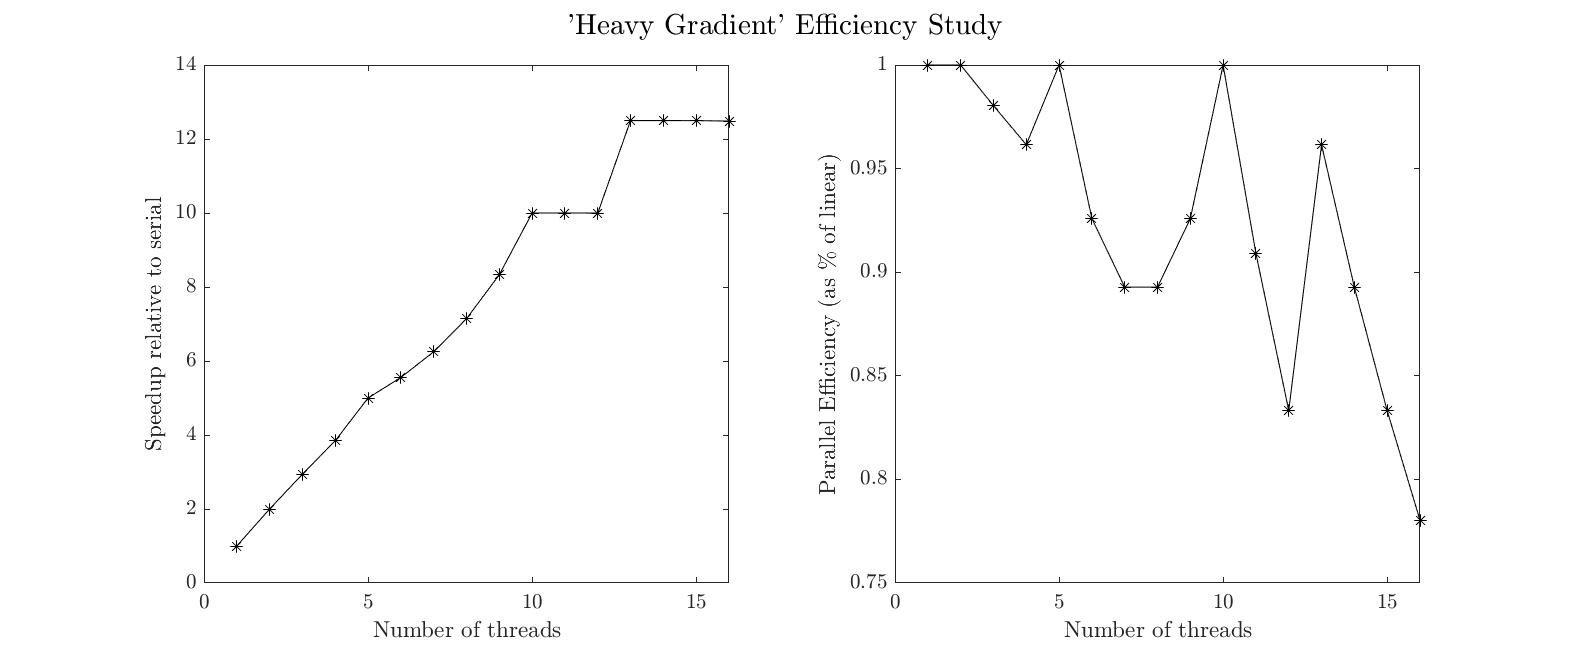
\includegraphics[width=\textwidth]{./resources/heavy_gradient}
  \caption{
  } \label{fig:heavygrad}
\end{figure}
